Слот (Slot<Args...>) --- это абстрактный вызываемый объект вида void (Args...), передающийся в качестве параметра

Виды Слотов:
\begin{itemize}
	\item Указатель на Функцию
	\begin{lstlisting}
		template <typename...Args>
		struct FunctionDelegator{
			void (*Function) (Args...);
		};
	\end{lstlisting}
	\item Указатель на функцию член класса и экземпляр класса
	\begin{lstlisting}
		template <typename...Args>
		struct ClassDelegator{
			SomeClass * Reciever;
			void (SomeClass::*Function) (Args...);
		};
	\end{lstlisting}
	\item Лямбда функция (Тело лямюды и указатель на функцию оператора вызова)
	\begin{lstlisting}
		template <typename...Args>
		struct LambdaDelegator{
			LambdaBody_type LambdaBody;
			void (LambdaClass::*Function) (Args...);
		};
	\end{lstlisting}
\end{itemize}

Задание (Task<Args...>) --- это Слот и аргументы, с которвми он должен быть вызван.

Сигнал (Signal) --- это лист из Слотов, которые вызываются при наступлении события, вызывающего сигнал. (Signal<Args...>)
Может быть 2 вида сигналов: 
\begin{itemize}
	\item Прямой (Direct) --- Вызов сигнала приводит непосредственно к вызову слота 
	\item Запланированный (Sheduled) --- вызов сигнала составляет Task, который добавляется в цикл обработки событий.
\end{itemize}

Эквивалентность Task<Args...> и Slot<>: Задание Task<Args...> эквивалетно Слоту типа Lambda. Функция вложения (гомоморфизм) будет следующей:
\begin{lstlisting}
	template <typename SlotType,typename...Args>
	auto make_task(SlotType Slot,Args...args){
		return [=](){return Slot(args...);};
	}
\end{lstlisting}


Система Сигналов и слотов:
Для реализации системы сигналов и слотов необходимо:
\begin{itemize}
	\item Хранить все соединенные слоты
	\item Хранить все задания (Task)
	\item иметь очередь заданий
	\item цикл обработки событий: примерная реализация следующая:
	\begin{lstlisting}
		while(!error_occured){
			if(!task_queue.empty() ){
				call(task_queue.pop_first());
			}else{
				sleep();	
			}
		}
	\end{lstlisting}
\end{itemize}
Если для хранения очереди заданий достаточно статического массива необходимой длины, то для хранение Слотов нужна динамическая аллокация. Однако для систем с малой памятью.

Возможно, наилучший способ --- иметь единое пространство для линамической аллокации, не подверженное фпагментации.

\subsection{структура microset}
Для динамической аллокации будем использовать страницы размером $N$ байт. Соответствующая структура эквивалетна классу \begin{lstlisting}
	T = std::array<char,N>
\end{lstlisting}

Для управления страницами будем использовать битовую маску. В итоге получается структура памяти
\begin{lstlisting}
	template <typename T,size_t _size>
	struct micro_set{
		T data[_size];
		bitmask_t mask;
	};
\end{lstlisting}

Для выделения памяти необходимо найти минимальный ненулевой бит (1 = ячейка свободна) в mask и вернуть его номер и присвоит ему 0, а для освобождения памяти необходимо соответствующий бит вернуть в состояние 1.

Для реализации битовой маски неоюходимо иметь класс целых чисел с длиной compile-time.
\begin{lstlisting}
	template <typename size_type,size_t length>
	struct bitmask_type;
\end{lstlisting}

Для осуществления контроля памяти необходимо уметь:
\begin{itemize}
	\item искать как можно быстрее единичный бит.
	\item выставлять бит в 0 или в 1.
\end{itemize}


\begin{table}[ht]
	\begin{center}
		\begin{tabular}{|c|c|}
			\hline
			Битовая маска & 
			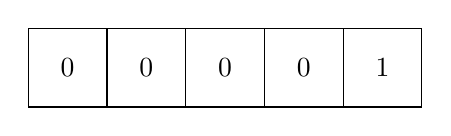
\begin{tikzpicture}
				\def\rectnum{5}
				\def\squaresize{1}
				
				 \foreach \i in {1,...,\rectnum} {
				 	 \pgfmathtruncatemacro\value{random(0,1)}
				 	 \ifnum\value=0
				 	 	\def\text{0}
				 	 \else
				 	 	\def\text{1}
				 	 \fi
				 	 \draw (\i*\squaresize, \squaresize) rectangle ++(\squaresize, -\squaresize)
				 	 node[midway] {\text};
				 }
			\end{tikzpicture}\\
			\hline
			
		\end{tabular}
	\end{center}
\end{table}






